% --------------------------------------------------------------
% This is all preamble stuff that you don't have to worry about.
% Head down to where it says "Start here"
% --------------------------------------------------------------
 
\documentclass[12pt]{article}
 
\usepackage[margin=1in]{geometry} 
\usepackage{amsmath,amsthm,amssymb}
\usepackage{listings}
\usepackage{graphicx}
\graphicspath{ {./images/} }

\lstset{
   basicstyle=\fontsize{8}{9}\selectfont\ttfamily
}
 
\newcommand{\N}{\mathbb{N}}
\newcommand{\Z}{\mathbb{Z}}
 
\newenvironment{theorem}[2][Theorem]{\begin{trivlist}
\item[\hskip \labelsep {\bfseries #1}\hskip \labelsep {\bfseries #2.}]}{\end{trivlist}}
\newenvironment{lemma}[2][Lemma]{\begin{trivlist}
\item[\hskip \labelsep {\bfseries #1}\hskip \labelsep {\bfseries #2.}]}{\end{trivlist}}
\newenvironment{exercise}[2][Exercise]{\begin{trivlist}
\item[\hskip \labelsep {\bfseries #1}\hskip \labelsep {\bfseries #2.}]}{\end{trivlist}}
\newenvironment{reflection}[2][Reflection]{\begin{trivlist}
\item[\hskip \labelsep {\bfseries #1}\hskip \labelsep {\bfseries #2.}]}{\end{trivlist}}
\newenvironment{proposition}[2][Proposition]{\begin{trivlist}
\item[\hskip \labelsep {\bfseries #1}\hskip \labelsep {\bfseries #2.}]}{\end{trivlist}}
\newenvironment{corollary}[2][Corollary]{\begin{trivlist}
\item[\hskip \labelsep {\bfseries #1}\hskip \labelsep {\bfseries #2.}]}{\end{trivlist}}
 
\begin{document}
 
% --------------------------------------------------------------
%                         Start here
% --------------------------------------------------------------
 
%\renewcommand{\qedsymbol}{\filledbox}
 
\title{Homework 1}%replace X with the appropriate number
\author{Hai Nguyen\\ %replace with your name
STAT760 - Statistical Learning} %if necessary, replace with your course title
 
\maketitle
 
\textbf{Problem 1}
\\Train a neareast neighbor classifier for handwritten digits with the training set provided, and test if using the test set.

\begin{itemize}
\item \textit{Source code (Python3):
}
\begin{lstlisting}[language=Python]
import numpy as np
from collections import Counter

# Function to return the major voted ID
def voting(lst):
    data = Counter(lst)
    return data.most_common(1)[0][0]

# Calculate the euclidean distance
def compute_distance (list_a, list_b):
	temp_arr = np.asarray(list_a) - np.asarray(list_b)
	return np.linalg.norm(temp_arr)

def kNN_classify(new_data_point, training_list, k, verbose):
	distance_list = []
	for i in range(len(training_list)):
		distance = compute_distance(new_data_point[1:], training_list[i][1:])
		distance_list.append([training_list[i][0], distance])
		# print(distance)
	sorted_list = sorted(distance_list, key = lambda x: x[1])

	result_list = [int(item[0]) for item in sorted_list[:k]]
	predicted_id = voting(result_list)
	correct_id = int(new_data_point[0])

	if (verbose):
		print("Predicted: ", predicted_id, "Correct Label:", correct_id)

	if (predicted_id == correct_id):
		return True
	else:
		return False

training_list = []
with open('zip.train') as f:
    for line in f:
        total_vec = line.split()
        total_vec = [float(i) for i in total_vec]
        training_list.append(total_vec)


# Open test file
f = open('zip.test')

# Changing k from [1-3] to see the difference
total_sample = 0
accuracy_cnt_max = 0
accuracy_cnt = 0
for k in range(1,4):
	f = open('zip.test')
	accuracy_cnt = 0
	total_sample = 0
	for line in f:
		total_sample += 1
		new_data = line.split()
		new_data = [float(i) for i in new_data]
		result = kNN_classify(new_data, training_list, k, False)
		if result:
			accuracy_cnt += 1

	print("k: ", k, "accuracy:", accuracy_cnt / total_sample * 100, "%")

	if (accuracy_cnt > accuracy_cnt_max):
		accuracy_cnt_max = accuracy_cnt
		k_optimal = k


print("Best k in [1,2,3] is ", k_optimal, "accuracy", accuracy_cnt_max / total_sample * 100, "%")

\end{lstlisting}
\item \textit{Outputs when ranging k from 1 to 3}
\begin{lstlisting}
k:  1 accuracy: 94.36970602889886 %
k:  2 accuracy: 93.17389138016941 %
k:  3 accuracy: 94.46935724962631 %
Best k in [1,2,3] is 3 accuracy 94.46935724962631 %
\end{lstlisting}

\end{itemize}
\textbf{Problem 2}

\begin{enumerate}
    \item For each of parts (a) through (d), indicate whether we would generally expect the performance of a flexible statistical learning method to be better or worse than an inflexible method. Justify your answer:

\begin{itemize}
    \item The sample size $n$ is extremely large, and the number of predictors $p$ is small. \\\textit{A flexible model can perform better as it can learn better from a large source of data points. Having many samples also reduces the possibility to be overfitting.}
    \item The number of predictors $p$ is extremely large, and the number of observations $n$ is small. \\\textit{A inflexible method would perform better as a flexible model would be prone to overfitting and the pattern picked up by it might be pure noise.}
    \item The relationship between the predictors and response is highly non-linear. \\\textit{Performance of a flexible statistical learning method is better as an inflexible method can only produce just a relatively small range of shapes to estimate $f$.}
    \item The variance of the error terms, i.e. $\mu^2 = \text{Var}(\epsilon)$, is extremely high.
    \\\textit{As the variance of the error terms is high, there is likely much noise in the data. Therefore, we prefer inflexible methods.}
\end{itemize}

\item Explain whether each scenario is a classification or regression problem, and indicate whether we are most interested in inference or prediction. Finally, provide $n$ and $p$.
\begin{itemize}
    \item We collect a set of data on the top 500 firms in the US. For each firm we record profit, number of employees, industry and the CEO salary. We are interested in understanding which factors affect CEO salary.
    \\\textit{This is a regression problem as the CEO salary is a continuous variable. We are interested in inference as we wish to know which factors will affect CEO salary. $n=500$ and $p=3$.}
    \item We are considering launching a new product and wish to know whether it will be a \textit{success} or a \textit{failure}. We collect data on 20 similar products that were previously launched. For each product we have recorded whether it was a success or failure, price charged for the product, marketing budget, competition price, and ten other variables.
    \\\textit{This is a classification problem as we want to classify a product is a success or a failure (discrete values). In this problem, we want to predict whether the new product will be successful or not based on the estimation of the underlying reliance of the success of past products on different factors. $n=20$ and $p=13$. }
    \item We are interested in predicting the \% change in the USD/Euro exchange rate in relation to the weekly changes in the world stock markets. Hence we collect weekly data for all of 2012. For each week we record the \% change in the USD/Euro, the \% change in the US market, the \% change in the British market, and the \% change in the German market.
    \\\textit{This is a regression problem as we want to predict a continuous value (\% change in the USD/Euro). We are interested in prediction in this percentage based on other weekly changes in the world stock markets. $n=52$ and $p=3$}
\end{itemize}

\item We now revisit the bias-variance decomposition.

\begin{itemize}
    \item Provide a sketch of typical (squared) bias, variance, training error, test error, and Bayes (or irreducible) error curves, on a single plot, as we go from less flexible statistical learning methods towards more flexible approaches. The x-axis should represent the amount of flexibility in the method, and the y-axis should represent the values for each curve. There should be five curves. Make sure to label each one.
    
    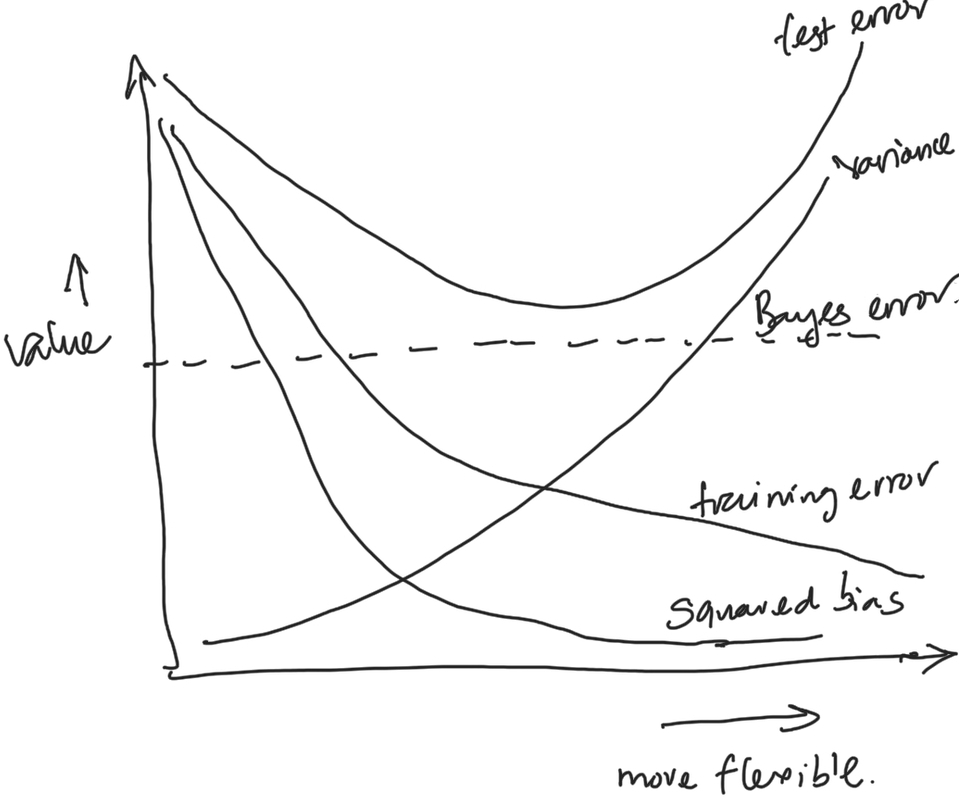
\includegraphics[scale=0.3]{images/cropped.jpeg}
    
    \item Explain why each of the five curves has the shape displayed in part (a).
    \\\textit{Bayes error is irreducible therefore it is constant regardless of the flexibility of the model used. Test error is always greater than Bayes error and when the model is more flexible, we are more likely to overfit the data, therefore test error is increasing. Also because of overfitting, training error is reducing. The sweet spot is when test error is minimum. When the model is more flexible, it has an increasing variance but a decreasing squared bias.}
\end{itemize}

\end{enumerate}


 
% --------------------------------------------------------------
%     You don't have to mess with anything below this line.
% --------------------------------------------------------------
 
\end{document}